\subsection[Scenariusz - man in the middle (Michał Krakowiak)]{Scenariusz - man in the middle}
Jednym z powszechniejszych zagrożeń sieciowych jest tzw. \textit{man in the middle}, czyli w dosłownym tłumaczeniu \textit{człowiek w środku}.
W takim scenariuszu napastnik pośredniczy w połączeniu internetowym danego systemu komputerowego.
W związku z tym wszystkie wysyłane i odbierane mogą być przechwycone oraz potencjalnie zmodyfikowane.
Tworzy to niebezpieczeństwo m.in. kradzieży ciasteczek, dodania kodu javascript do zapytania oraz bardziej zaawansowanych ataków na połączenia szyfrowane jak SSLsplit.
\subsubsection[Aktorzy]{Aktorzy}
\begin{itemize}
    \item Pentester – osoba przeprowadzająca test bezpieczeństwa systemu komputerowego za pomocą dedykowanego systemu
    \item Urządzenie wykonujące – niewielkie urządzenie oparte o platformę Raspberry Pi Zero W, podłączone za pomocą portu USB do testowanego systemu
    \item Serwer sterujący – centralny punkt infrastruktury, rejestruje aktywne urządzenia wykonujące, przyjmuje polecenia od testera, przekazuje je do wskazanych urządzeń wykonującyc.
    \item Testowany system – system komputerowy pracujący pod kontrolą systemu operacyjnego Windows 10, użytkownik nie posiada uprawnień administratora
\end{itemize}
\subsubsection[Przebieg]{Przebieg}
Test bezpieczeństwa korzystający realizowanego systemu rozpoczyna się od dostarczenia i instalacji skonfigurowanego urządzenia wykonującego.
Uruchomiony system komputerowy dostarczy zasilanie urządzeniu po przez port USB.
Podczas swojego startu urządzenie wykonujące uruchamia skrypt odpowiedzialny za obsługę komunikacji z serwerem sterującym oraz obsługę połączenia USB.
Resztę działań tester przeprowadza zdalnie. Z poziomu przeglądarki ma dostęp do aplikacji która pozwala wskazać jedno lub więcej urządzeń zarejestrowanych w systemie.
Następnie przygotowuje odpowiedni dla testu payload, w którym wskazuje takie elementy jak:
\begin{itemize}
    \item tryb działania: tylko podsłuch czy wstrzykiwanie kodu
    \item ilość datagramów IP, które mają zostać podsłuchane
    \item kod html lub javascript, który zostanie dołączony do określonej liczby odpowiedzi HTTP
\end{itemize}
Po poprawnym przyjęciu żądanej operacji serwer sterujący wysyła wiadomość z ładunkiem do wskazanych urządzeń.
Identyfikują one polecenie i rozpoczyna wykonywanie skryptów inicjujących wymagane funkcjonalności. Uwzględnia to ewentualną zmianę z innych zrealizowanych trybów pracy.
Urządzenie wykonujące rejestruje swoją obecność w testowanym systemie komputerowym jako zewnętrzna karta sieciowa.
Następnie rozsyłane są odpowiednio spreparowane ustawienia DHCP dla nowo przyłączonego interfejsu sieciowego w testowanym systemie.
Zapewniają, że ruch sieciowy będzie kierowany na spreparowaną kartę sieciową, a następnie obsługiwany w żądany sposób.
Sposób działania urządzenia powinien być możliwie transparentny.
\begin{figure}[H]
    \centering
    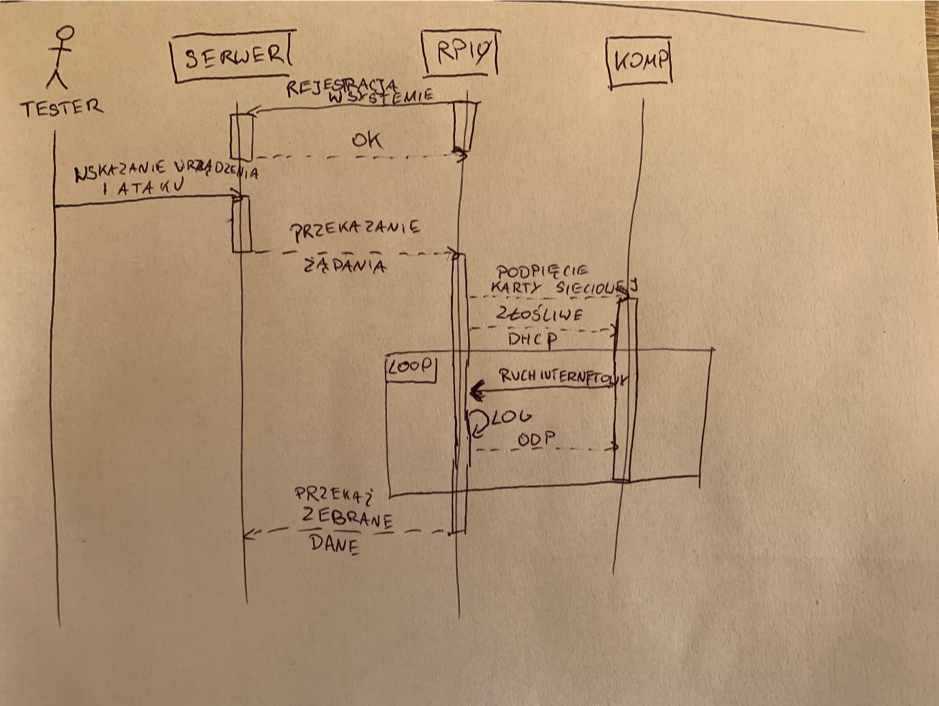
\includegraphics[width=\textwidth]{mk05}
    \caption{Mitm}
    \label{fig:mitm}    
\end{figure}